\documentclass{article} % For LaTeX2e
\usepackage{nips15submit_e,times}
\usepackage{hyperref}
\usepackage{url}
\usepackage{lineno}
\usepackage{graphicx}
\usepackage{amsmath}
\usepackage[all]{hypcap} 
%\linenumbers% Uncomment for line numbers



\title{America's Warzone: Predicting Gun Violence in Chicago}

\author{
Reuben K. McCreanor\thanks{Department of Statistical Science, Duke University} \\  
\texttt{reuben.mccreanor@duke.edu} \\
\And
Anna Yanchenko\footnotemark[1] \\
\texttt{anna.yanchenko@duke.edu} \\
\And 
Lei Qian\footnotemark[1] \\
\texttt{lei.qian@duke.edu} \\
\And
Megan Robertson\footnotemark[1] \\
\texttt{megan.robertson@duke.edu} \\ 
}

\hypersetup{
    colorlinks=true,
    linkcolor=blue,
    filecolor=magenta,      
    urlcolor=cyan,
    pdftitle={Sharelatex Example},
    bookmarks=true,
    pdfpagemode=FullScreen,
}


\newcommand{\fix}{\marginpar{FIX}}
\newcommand{\new}{\marginpar{NEW}}

\nipsfinalcopy 

\begin{document}

\maketitle

\begin{abstract}
In 2008, of the 7 million flights within the United States, more than 23\% arrived at least 15 minutes late. Specifically, we examine which days of the week and major airports are optimal to fly from in order to minimize delays, whether delays vary significantly by carrier, and whether delay is related to the magnitude of a carrier's presence in major airport hubs throughout the United States. In general, we find that flights departing on Mondays and Thursdays experience less delay than flights departing on other days of the week, that there is no statistically significant difference in delay between airlines, and that airlines with a major presence in a specific airport experience less delays than other airlines in the same airport.
\end{abstract}

\section{Introduction}
\label{headings}

Each day, there are approximately 28,000 commercial flights in the United States \hyperlink{Ref2}{[2]}. On a daily basis, an average of 8,363 of these flights will be delayed \hyperlink{Ref1}{[1]}. The economic cost of these delays includes increased fuel and maintenance costs for airlines, a decrease in economic efficiency from lost passenger time, and the welfare loss incurred by passengers who avoid air travel because of delays. The direct cost of flight delays in the United States in 2007 was estimated to be more than \$28 billion \hyperlink{Ref3}{[3]}. 

For this reason, we seek to determine which variables influence arrival delay. First, we explore which factors under the passenger's control are most important in predicting arrival delays. This question will consider factors such as time and day of the week that a flight departs, the distance of the flight and what city the flight departs from. Second, we explore whether some carriers experience more delays than other carriers. As the choice of airline is one of the main variables under a passenger's control, any airline that experiences comparatively more delays would be a clear one to avoid. Finally, we consider whether a strong carrier presence within a specific airport influences delays compared to airlines with a smaller presence in the same airport. That is, do airlines experience preferential treatment in their airport hubs in terms of reducing flight delays?   We seek to answer these questions using a combination of Bayesian and Frequentist methods on over 7 million flights for the year 2008 \hyperlink{Ref1}{[1]},\hyperlink{Ref5}{[5]},\hyperlink{Ref6}{[6]}.  

\section{Discussion of Methods}
\label{headings}

We approach each of our three questions separately, utilizing specific techniques for each analysis. 

To answer the question of which passenger controlled factors are important predictors for arrival delays, we perform Frequentist regression analysis and include nineteen variables in the three models considered: ordinary least squares (OLS), LASSO, and Ridge Regression. Please see \ref{appendix_regression} for a detailed discussion of regression methods and variable selection. 
 
To explore whether arrival delay varies by carrier, we utilize Bayesian inference methods (\ref{appendix_bayes}). We calculate posterior means and 95\% credible intervals for the proportion of flights delayed, the mean delay in minutes and the standard deviation of the delay for individual carriers. Additionally, we use Monte Carlo methods to estimate differences in these quantities between airlines. Finally, we utilize Bayesian hypothesis testing to compare the proportion of flights delayed for one airline compared to another. 

Finally, to examine the relationship between carrier presence and delay, we create a subset of 1,114,510 flights and 464 variables to include only observations with a positive departure delay. Variable selection is performed via OLS and 130 variables that fail a 90\% significance criteria are removed. We then perform a second-stage OLS on each departure delay metric and plot the fitted curve for each iteration of each model for airline presence percentages between 0\% and 70\% at specific airports. For further discussion on this method, please see \ref{appendix_hub}.

\section{Results}
\label{headings}

\subsection{Predicting Airline Delay}

For our exploration of which passenger controlled factors are important predictors for arrival delays, all three regression methods yield consistent results, both in terms of MSE values and coefficient estimates. OLS and LASSO regressions have identical, highly significant MSE values, while Ridge regression has a slightly higher, though still significant, MSE value. In terms of variable selection, the OLS and LASSO regression methods find that the Tuesday indicator variable is not significant. The OLS model additionally finds that the Wednesday, Los Angeles and Las Vegas indicator variables are not significant in predicting arrival delay. The adjusted $R^2$ value for the OLS regression model is 0.6344, indicating that 63\% of the variation in arrival delay is explained by variation in the predictor variables in our model.

The coefficient estimates from all three methods are quite similar in magnitude (\autoref{coef_values}). Coefficients with negative values indicate that holding all other variables constant, a one unit increase in the considered variable results in a decrease in arrival delay.  

Based on our coefficient estimates, flights departing on Sunday or Friday have a larger delay than flights departing during the rest of the week. This result makes sense, as on Sundays, there are many flights with people leaving for the workweek and returning from the weekend, while on Friday, people are both returning home after the workweek and leaving for the weekend. Based on the coefficient estimates, Thursday is the best day to fly, as it has the highest magnitude negative coefficient among the days of the week. These coefficient estimates are in reference to Saturday, so Sunday, Friday and Wednesday are worse days to fly for delays than Saturday, and Monday and Thursdays are better in terms of having a smaller delay.

The coefficients for the flight origin airport are calculated in reference to San Francisco. Compared to San Francisco, flights leaving from Atlanta, Orlando, Dallas Fort-Worth, JFK, Houston and Charlotte have, on average, smaller delays, while Los Angeles, Las Vegas and Phoenix have, on average, longer delays than San Francisco.  

Several regression models were considered and in nearly all of them, the departure delay was a very important variable in increasing the prediction accuracy of the model. When we dropped departure delay from considered models, our MSE increased significantly and the adjusted $R^2$ decreased to 1\%. Intuitively, if a flight has a large departure delay, the arrival delay is expected to be large as well, so it makes sense that departure delay is the single largest predictor of arrival delay.

\subsection{Aggregate Delay Difference between Carriers}

The Shiny app for Bayesian analysis allows the user to analyze each of the 20 unique carriers in our data and compare any two airlines \hyperlink{Ref7}{[7]}. For example, we compare delays for American Airlines to delays for Delta Airlines \autoref{bayes_plots}. We find that while the mean delay is essentially the same for American and Delta, American has a higher proportion of flights delayed than Delta, and a higher standard deviation for delayed flights than Delta.  

Bayesian hypothesis testing results confirm the Monte Carlo results for the difference in proportion of flights delayed. The probability of that the proportion of flights delayed for American and Delta is different is 0.9999448 with a Bayes Factor of 18,100 in favor of this alternative hypothesis. Thus, there is very strong evidence in favor of the alternative hypothesis and we can conclude that the proportion of flights delayed for American Airlines and the proportion delayed for Delta is indeed different.

\begin{figure}[h]
\begin{center}

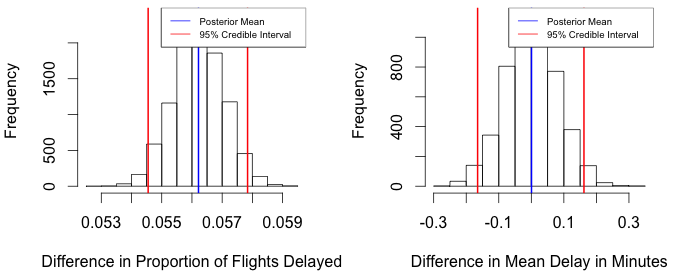
\includegraphics[width=0.8\textwidth,keepaspectratio]{bayes_plots.png}
\caption{Histogram of the Monte Carlo simulated difference in mean delay and proportion of flights delayed more than 15 minutes between American Airlines and Delta (i.e. American - Delta). The mean difference in the proportion of flights delayed is about 0.0562 and the probability that the proportion of flights delayed for American is more than the proportion delayed for Delta is 1. While only about 5\% more flights are delayed for American than for Delta, there is always a higher proportion of American flights delayed than Delta flights. The posterior mean for the difference in the mean delay in minutes for America and Delta is 0, with probability 0.4976 that the mean delay for American is greater than the mean delay for Delta. Thus, there is statistically no significant difference in the mean delay for American flights compared to Delta flights. Finally, the standard deviation of flight delays is about 8.75 minutes more for American Airlines compared to Delta, with a probability of 0.98 that the standard deviation for American delays is greater than the standard deviation for Delta delays.}
\label{bayes_plots}
\end{center}
\end{figure}
 
\subsection{The Effect of Substantial Airline Presence}

Using a two-stage OLS regression approach, we find a significant, non-linear relationship between airline presence at an airport and average departure delay length. Specifically, given that a flight is delayed on departure, an airline that operates 40\% of flights in a given airport is expected to have an average departure delay of approximately 21 minutes less than an airline that operates 1\% of local flights. The corresponding gain for an airline that operates 25\% of flights is approximately 9.3 minutes. We conclude that these figures are substantial and confirm the existence of strong majority-hub bias. However, it is difficult to speculate about the direction of this relationship, as carriers operate more efficiently and enjoy economies of scale in majority hubs, while airport management may reciprocally offer preferential treatment to their largest customers.

\begin{figure}[h]
\begin{center}

\includegraphics[width=0.9\textwidth,keepaspectratio]{carrier_presence.png}
\caption{Fitted curves between presence and departure by type of delay. Air carrier delays are due to circumstances under the airline's control, weather delays are a result of actual or forecasted significant meteorological conditions and NAS delays are determined by the national aviation system and include heavy traffic volume, non-extreme weather and air traffic control. Late-arriving aircraft and security delays are a result of a previous flight arriving behind schedule and delays as a result of airport security, respectively. [8]\label{carrier_plot}}

\end{center}
\end{figure}

Breaking delay times down by category provides some insight \autoref{carrier_plot} into this question. With the exception of security delay times, all delay time-presence relationships have significant higher-order terms up to the 6th power. Weather delay times drop gradually as presence increases from 0\% to 70\%, suggestive of efficiency and the availability of contingency options leading to robust gains in punctuality. Evidence for preferential treatment is less concrete, but can perhaps be observed from National Air System (NAS) delays, which drop sharply only between zero and approximately 5\% presence and beyond 60\%. This could be partially attributed to a necessary critical mass of carrier presence required for effective management and rescheduling. It may, however, also be caused in part by airports prioritizing sufficiently important carriers over ones with significantly less presence.

For an example of predicted delay reduction, \autoref{carrier_table} compares expected departure delay times, given delay existence, of carriers by airport. Each of the four carriers have a major hub among the four airports: Delta in Atlanta, American Airlines in Dallas-Fort Worth, United in Denver, and US Airways in Charlotte. Holding other factors constant, we can observe that in all four cases, the estimated major presence benefit is substantial: compared to United, for example, Delta flights in Atlanta are expected to enjoy delay reductions of 19.6 minutes on average. Conversely, in Denver, United flights are expected to enjoy delays of 7.1 minutes less than Delta flights. 

\begin{table}[ht]
\centering
\begin{tabular}{rrrrr}
  \hline
 & Delta & American & United & US Airways \\ 
  \hline
Atlanta & \bf{46.1} & 61.8 & 65.7 & 64.6 \\ 
  Dallas-FW & 64.1 & \bf{52.7} & 64.1 & 62.1 \\ 
  Denver & 63.9 & 62.3 & \bf{56.8} & 64.4 \\
  Charlotte & 65.3 & 67.2 & 66.9 & \bf{57.1} \\ 
   \hline
\end{tabular}
\caption{Average Delay Time (min.) for Carrier in Airport - minimum delay is bolded.\label{carrier_table}
}

\end{table}


\section{Conclusion}
\label{headings}


In conclusion, we find that there is no single airline that outperforms other airlines in terms of minimum arrival delays. All airlines suffer from significant delays, and the best strategy for minimizing delays is dependent on the time of travel, the destination and the carrier presence in the destination airport. In terms of designing an optimal flying strategy, our results indicate that Mondays and Thursdays are the best days to fly for minimum arrival delays, departing from Atlanta, Orlando, Dallas, JFK, Houston or Charlotte is preferable to departing from San Francisco, Los Angeles, Las Vegas or Phoenix and that there is a benefit to traveling from a specific airline's hub in terms of reducing delays. Further analysis would include the addition of data about more airlines and more destinations in the regression analysis and also would utilize outside data, such as weather records for each day, to more accurately predict arrival delay. Additionally, trends in the secondary airport hubs for major carriers would be explored to determine if these smaller hubs experienced the same delay trends as the airline's main hub.  

\clearpage
\newpage


\subsubsection*{References}


\hypertarget{Ref1}{[1] American Statistical Association. \textit{Data Expo 2009}. Statistical Computing and Statistical Graphics. Accessed October 20, 2015. \url{http://stat-computing.org/dataexpo/2009/the-data.html}.}

\hypertarget{Ref2}{[2]} National Oceanic and Atmospheric Administration. \textit{Air Traffic}. Science on a Sphere. Accessed October 30, 2015. \url{http://sos.noaa.gov/Datasets/dataset.php?id=44}.

\hypertarget{Ref3}{[3]} Ball, Michael et. al. \textit{Total Delay Impact Study: A Comprehensive Assessment of the Costs and Impacts of Flight Delay in the United States}. The National Center of Excellence for Aviation Operations Research (NEXTOR), October 2010.

\hypertarget{Ref4}{[4]} Socrata. \textit{Airport Codes mapped to Latitude and Longitude in the United States}. Open Data. Accessed November 10, 2015. \url{https://opendata.socrata.com/dataset/Airport-Codes-mapped-to-Latitude-Longitude-in-the-/rxrh-4cxm}.

\hypertarget{Ref5}{[5]}United States Department of Transportation. \textit{On-Time Performance}. Bureau of Transportation Statistics. Accessed November 15, 2015. \url{http://www.transtats.bts.gov/Fields.asp?Table_ID=236}.

\hypertarget{Ref6}{[6]}American Statistical Association. \textit{Data expo 2009 Supplementary Data}. Statistical Computing and Statistical Graphics. Accessed November 14, 2015. \url{http://stat-computing.org/dataexpo/2009/supplemental-data.html}.

\hypertarget{Ref7}{[7]} Link for Shiny App: \url{https://reuben.shinyapps.io/Flight_Dealys}.

[8] United States Department of Transportation. \textit{Understanding the Reporting of Causes of Flight Delays and Cancellations}. Bureau of Transportation Statistics. Accessed November 20, 2015. \url{http://www.rita.dot.gov/bts/help/aviation/html/understanding.html}.

\hypertarget{Ref9}{[9]} Federal Aviation Administration. \textit{Types of Delay}. Accessed November 18, 2015 \url{http://aspmhelp.faa.gov/index.php/Types_of_Delay}.

\clearpage
\newpage

\section{Appendix}
\label{headings}


\subsection{OLS, LASSO and Ridge Regression Methods}
\label{appendix_regression}

Of the 29 original variables in the data set, we initially select only variables of interest for predicting arrival delay. These variables are the day of the week, CRS departure time, airline carrier, origin, destination, departure delay, and flight distance. We then further subset the data to only look at four specific carriers, Delta, American Airlines, United Airlines and US Airways.  Each of these airlines flew approximately 7-8\% of domestic flights in 2008 and are the four airlines considered in our hub delay analysis. We do not include an indicator for the carrier, as we find in our Bayesian analysis that there is not a significant difference in the mean delay for these four carriers.  

We further subset the data to only look at flights originating in one of the 10 largest airports by number of flights in 2008. These airports, in order, are Atlanta, Orlando, Los Angeles, Dallas Fort-Worth, JFK, Las Vegas, Houston, Phoenix, Charlotte and San Francisco. We add nine indicator variables indicating whether a flight has originated in one of these cities (value = 1) or not (value = 0), with San Francisco as the reference level. We additionally add one indicator variable for the destination of the flight; this variable has a value of 1 if the destination is one of these 10 largest airports and 0 otherwise. Finally, we add six indicator variables for each day of the week, with Saturday as the reference level.  The CRS Departure time is treated as a continuous variable.  

The arrival delays were highly right skewed, thus we remove flights with a delay of less than 15 minutes and an arrival delay of more than 180 minutes and take the natural log transformation of the arrival delay. We then perform exploratory data analysis (specifically, we find the transformation plot for symmetry) to further transform the arrival delay to make the distribution more symmetrically distributed and to improve the residual distribution in our model fits.  
 
Three regression methods are performed with the variables selected above: ordinary least squares regression (OLS), LASSO and Ridge regression. For both the LASSO and Ridge regressions, 10-fold cross validation is used to select a penalty parameter that corresponded to the minimum MSE value for the model. Diagnostics are performed for the regression models and the model assumptions are fairly well met (\autoref{diagnostics}). There are some large residual values and some divergence from normality of the residuals near the lower tail, though constant variance of the residuals and independence of residuals are well satisfied. The LASSO and Ridge regressions are run with the data standardized. The models are trained on 151,324 observations and tested on 37,831 observations (80\% training data to 20\% testing data split). Coefficient estimates for the three methods considered are in \autoref{coef_values} below.
 
 \begin{table}[ht]
 
\centering
\begin{tabular}{rrrr}
  \hline
 & OLS & LASSO & Ridge  \\ 
  \hline
(Intercept) & 6.650E-01 & 6.643E-01 & 6.608E-01 \\ 
  CRSDepTime & 1.425E-06 & 1.312E-06 & 5.958E-07 \\ 
  DepDelay & -7.811E-04 & -7.796E-04 & -7.157E-04 \\ 
  Distance & -2.981E-07 & -1.850E-07 & -1.187E-07 \\ 
  Dest & -2.633E-03 & -2.494E-03 & -2.288E-03 \\ 
  ATL & -3.755E-03 & -2.926E-03 & -1.028E-03 \\ 
  ORD & -5.291E-03 & -4.526E-03 & -3.395E-03 \\ 
  LAX & 2.166E-05 & 4.813E-04 & 1.403E-03 \\ 
  DFW & -3.532E-03 & -2.751E-03 & -1.255E-03 \\ 
  JFK & -1.118E-02 & -1.044E-02 & -8.482E-03 \\ 
  LAS & 3.039E-04 & 7.737E-04 & 1.749E-03 \\ 
  IAH & -4.083E-03 & -3.083E-03 & -2.064E-03 \\ 
  PHX & 9.597E-04 & 1.481E-03 & 2.714E-03 \\ 
  CLT & -4.063E-03 & -3.198E-03 & -1.291E-03 \\ 
  Sunday & 6.506E-04 & 5.325E-04 & 5.563E-04 \\ 
  Monday & -7.077E-04 & -6.675E-04 & -6.613E-04 \\ 
  Tuesday & -1.313E-05 & 0.000E+00 & 1.528E-04 \\ 
  Wednesday & 3.467E-04 & 2.359E-04 & 4.365E-04 \\ 
  Thursday & -1.054E-03 & -1.020E-03 & -1.035E-03 \\ 
  Friday & 1.237E-03 & 1.094E-03 & 1.105E-03 \\ 
   \hline
\end{tabular}
\caption{Coefficient Estimates for OLS, LASSO and Ridge Regression Methods\label{coef_values}} 

\end{table}
 
 


\begin{figure}[h]

\begin{center}
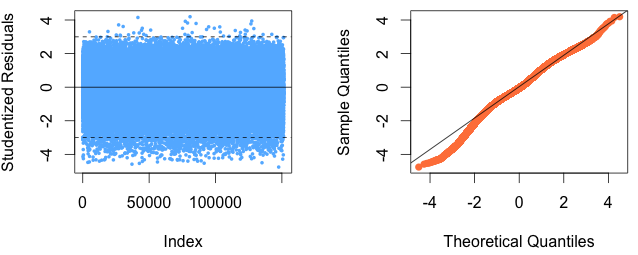
\includegraphics[width=\textwidth,height=\textheight,keepaspectratio]{model_diagnostics.png}
\caption{Studentized residuals and QQ plot of residuals from the OLS regression model\label{diagnostics}}

\end{center}
\end{figure}

\subsection{Bayesian Analysis Methods}
\label{appendix_bayes}



Our Shiny app allows users to interactively select which airlines they wish to explore, either individually or to compare to another airline\hyperlink{Ref7}{[7]}. We explore the posterior distributions of three different quantities for each airline, the proportion of flights delayed more than 15 minutes upon arrival, the mean delay of flights and the standard deviation of flight delays. Whether a flight is delayed for a specific airline by at least 15 minutes or not is a binary variable and can be modeled by Bernoulli($\theta$) distribution, where $\theta$ is the proportion of flights delayed. In order to have a conjugate posterior distribution, the prior distribution selected for $\theta$ is Beta(2,5). These Beta parameters are selected by finding that the majority of airlines experience arrival delays of more than 15 minutes approximately 20\% of the time. Beta(2,5) is peaked at 0.20 with most of the density concentrated between 0.1 and 0.4, corresponding to the range of the proportion of arrival delays for all carriers considered. With a Bernoulli($\theta$) likelihood and Beta(2,5) prior, the posterior distribution for $\theta$ is $\pi (\theta | X)\propto\mbox{Beta}(2+\sum_{i=1}^n X_i, n+5-\sum_{i=1}^n X_i)$, where $X_i$ is the binary variable for whether flight $i$ is delayed by more than 15 minutes or not and $n$ is the total number of flights for the carrier considered.   

To find the posterior distribution for the mean and standard deviation, we use a normal-inverse-gamma model as we desire conjugacy and the ability to utilize Gibbs sampling for our posterior estimates. We assume that the arrival delay for flights for a specific airline is approximately normally distributed. Though there is right skew for the arrival delay for all flights in 2008 considered, we have enough observations (approximately 7 million) to ensure that this assumption is reasonable. Considering only a specific airline carrier, we then have a normal likelihood for the data, 
$$L(Y | \mu, \tau) \propto \tau^{n/2}\mbox{Exp}(-\dfrac{1}{2}\tau \sum_{i=1}^n (Y_i - \mu)^2),$$ where $Y_i$ is the delay of flight $i$ in minutes, $\mu$ is the mean delay and $\tau$ is the precision or the inverse of the variance of flight delays.  Assuming priors of $\mu\sim N(\mu_0, \tau_0)$ and $\tau\sim\mbox{Gamma}(a,b )$, we find the full conditionals for $\mu$ and $\tau$ so that we can use Gibbs sampling for our posterior estimates. These full conditionals are $$\pi(\mu | Y, \tau)\propto N \Big( \dfrac{\mu_0\tau_0+\tau\sum_{i=1}^n Y_i}{\tau_0+\tau n}, (\tau_0+\tau n)^{-1}\Big)$$ and $$\pi(\tau | Y, \mu)\propto\mbox{Gamma}(a+\dfrac{n}{2}, b+\dfrac{1}{2}\sum_{i=1}^n (Y_i - \mu)^2),$$ respectively. In the Shiny app, the Gibbs sampler is run for 3000 iterations with a burn-in of 100 iterations. To choose the prior values $a$, $b$, $\mu_0$ and $\tau_0$, we again look at the data to determine reasonable choices for these values. When looking at all of the flights in 2008 for each airline, the majority of airlines have a standard deviation of approximately 30 minutes for their arrival delays. This means that the precision tends to be around 1/900, so we select $a=1$ and $b = 100$ for a prior distribution peaked around 1/900. For the values of $\mu_0$ and $\tau_0$, we use the mean delay and the standard deviation for all flights for the airline considered, respectively. The posterior mean and the 95\% credible interval for each parameter considered are calculated.

When the user wishes to compare the delays between two airline carriers, we use Monte Carlo methods to simulate distributions and probabilities of interest. For the proportion of flights delayed, the mean flight delay and the standard deviation of flights delayed, we first sample from the posterior distributions for airline 1 and airline 2 as outlined above. We then subtract each posterior estimate from airline 2 from the corresponding posterior estimate for airline 1 to obtain a Monte Carlo estimate of the distribution of the difference between the parameter of interest for airline 1 and airline 2. We additionally count the number of times that the parameter estimate for airline 1 is greater than the parameter estimate for airline 2 and divide by the total number of estimates considered to obtain a Monte Carlo estimate for the probability that the posterior parameter estimate for airline 1 is greater than the posterior parameter estimate for airline 2. 

Finally, when there are two airlines compared, we conduct Bayesian hypothesis testing to determine if the proportion of flights delayed by more than 15 minutes for airline 1 is the same or different as the proportion of flights delayed for airline 2.  Our null and alternative hypothesis are:
$$H_0: \theta_1 = \theta_2 = \theta$$
$$H_1: \theta_1 \neq \theta_2$$
where $\theta_1$ is the proportion of flights delayed more than 15 minutes for airline 1 and $\theta_2$ is the proportion of flights delayed more than 15 minutes for airline 2.  

We choose a 0-1 loss for our testing and assume prior probabilities of 0.5 on the null and alternative hypotheses being true, i.e. Pr(H0 true) = Pr(H1 true) = 0.5. The 0-1 loss function means that if the true state of nature is equal to the chosen hypothesis, then the loss is 0, but if the true state of nature is not equal to the chosen hypothesis, then the loss is 1.  

The probability of the alternative hypothesis being true is
$$Pr(\mbox{H1 true}) = 1 - \dfrac{1}{1+BF}$$ where BF is the Bayes factor in favor of H1.  The Bayes factor is equal to $\dfrac{L(data | \mbox{H1 true})}{L(data | \mbox{H0 true)}}$, where for our data specifically, 
$$L(data | \mbox{H0 true}) = \dfrac{B(\sum_{i=1}^{n_X}X_i + \sum_{i=1}^{n_Y}Y_i + a, n_Y +n_X -  \sum_{i=1}^{n_X}X_i - \sum_{i=1}^{n_Y}Y_i + b) }{B(a,b)}$$
$$L(data | \mbox{H1 true}) = \dfrac{B(\sum_{i=1}^{n_Y}Y_i + c, n_Y - \sum_{i=1}^{n_Y}Y_i +d) B(\sum_{i=1}^{n_X}X_i + e, n_X - \sum_{i=1}^{n_X}X_i +f)}{B(c,d)B(e,f)}$$

where B($\alpha$, $\beta$) is the Beta coefficient, $X_i$ and $Y_i$ is the data for airline 1 and 2, respectively on whether the flight is delayed by more than 15 minutes or not and where $a-f$ are prior parameters, i.e. $(\theta = \theta_1 = \theta_2 | \mbox{H0 true})\sim \mbox{Beta}(a,b)$ and $(\theta_1 |\mbox{H1 true})\sim \mbox{Beta}(c,d)$,    $(\theta_2 | \mbox{H1 true})\sim \mbox{Beta}(e,f)$.  As above, under H0 true, we selected $a=2$, $b=5$.  Under H1, we select the priors Beta(1.7, 5) for the airline with a lower proportion of delays and Beta(2.5, 5) for the other airline. These priors are chosen because they again concentrate most of the density around 0.20, but the maximum of Beta(1.7, 5) is shifted to the left of the maximum of Beta(2.5,5), so the priors are providing some information that we expect the  the airline with a lower proportion of flights delayed initially to also have a lower proportion of flights delayed in the posterior estimate under H1.  

\break
\begin{figure}[h]

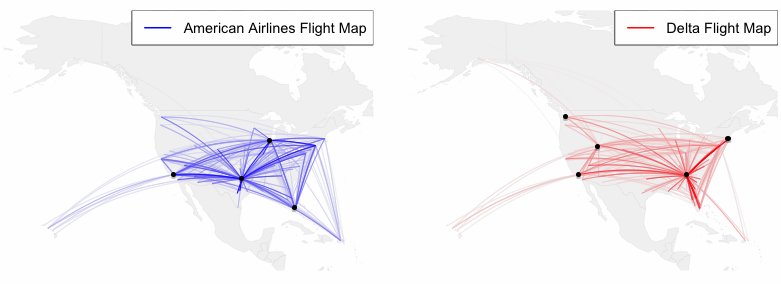
\includegraphics[width=\textwidth,height=\textheight,keepaspectratio]{flight_map}
\caption{Map of American Airlines and Delta flights throughout the United States (hubs as of 2008 indicated by points)[4]}

\end{figure}


\subsection{Carrier Presence Methods}
\label{appendix_hub}

As discussed in the paper the full model for carrier presence in major airline hubs is constructed with a full-observation, positive departure delay-only subset of 1,114,510 flight observations and 464 variables, including presence percentage in decimal and transformations up to the 6th power, flight time in minutes, indicators for carrier, airport, day-of-year, and delay and arrival time of day by hour-block. To achieve the delay-presence relationship estimates, we perform a two-stage OLS regression with an initial variable-selection process. Variable selection is performed via OLS with variables that fail a 90\% significance criteria, 130 in total, removed. OLS is chosen after testing a number of alternative penalization approaches, including forward stepwise via a 25,000-observation training set, elastic net, and LASSO with 10-fold cross-validation to similar conclusions. We hence concluded that the simple OLS model selection approach, in addition to speed benefits, is sufficient for the purpose of this investigation. 

A second-stage OLS is performed for each departure delay category, including the total delay time (DepDelay) and five delay-cause categories. For each metric, we subset the data to positive-values only for the dependent delay variable and performed 25 OLS iterations with a randomly-selected 20\% training set for each iteration. These multiples runs provide stabilized estimates of the parameters of interest (presence), test each model for observation-chasing of higher-order terms, and serve as confidence intervals. We plot the fitted curve for each iteration of each model for presence percentages between 0\% and 70\%. 

As shown in graph \autoref{carrier_plot}, all delay categories, with the exception of Security and Carrier delay, display clear, non-linear, downward-sloping trends. Distributions of different iterations generally lead to growing uncertainty for higher airline presence, but does not significantly alter the negative relationship. Predictions in some categories (weather, late aircraft delays) assume negative values at presence levels above 60\%, which is likely caused by very high-presence airlines having virtually no delays attributed to these categories, or are even regularly early, because of robust contingency or sufficiently large scale within an airport. A full discussion of the nuanced effects of airline presence on each delay type is possible given the low uncertainty of estimate, but beyond the scope of this paper. 

In \autoref{carrier_plot}, departure delay is calculated as the sum of the five delay categories (Carrier, Weather, NAS, Security, and Late Aircraft), as defined by the Federal Aviation Administration \hyperlink{Ref9}{[9]}. 



\end{document}


